\clearpage
\chapter{Introduction}
\label{sec:intro}
Performing experiments is a key component of human development and has been the foundation of knowledge gain during the evolution of mankind. However, the exchange of such experimental results requires the long term documentation of the  experimental procedure. This is only possible with the means of writing down the experimental purpose, execution and result in an exact, complete and unbiased fashion. Nowadays, tedious manual scripture has largely been replaced by digital information, making information easier to be transported, searched and duplicated. Therefore, scientific research nowadays relies mainly on digital information acquisition and storage. Although data can be easily stored and disseminated with modern technologies, interpretation of research data is not straight forward as datasets are highly diverse between and often even within scientific areas. The diversity within a field highly depends on the field, e.g., in fields which require large experimental setups (particle physics / high field FMRI) there are only a few data formats defined by the community / company producing the corresponding setup (e.g., the \code{root} format \citep{Brun_1996} and the NIfTI file format). In other fields the diversity of data is bigger since the scientific methods and aims require a diversity of approaches. Unification would require organizational large-scale efforts across the community and implies additional overhead on the level of each experiment. A number of initiatives try to screen, collect and evaluate community specific and community overarching data and metadata approaches. Some examples here are the Human Brain Project\footnote{HBP, \url{https://www.humanbrainproject.eu/en/}} (HBP), developing a platform for gathering neuroscientific data from all neuroscientific areas. A community overarching approach is a recent German initiative for systematic and sustainable research data management within and across disciplines (national research data infrastructure). However, often this top-down approach focuses on the few common features of datasets, where it is typically already a challenge to define a set of basic minimal metadata to superficially describe a dataset. Much less attention is devoted to the problem of obtaining an in-depth description of a specific dataset that is consistent with similar data. In light of the complexity of such in-depth metadata, a prerequisite is to provide tools and workflows for the implementation of sustainable data and metadata management on a laboratory level. This permits the integration of data and metadata on a detailed level in a standardized structure, which can later be integrated in large scale infrastructure projects.

The diversity in data modalities and file formats promotes also a heterogeneity in data analysis steps and tools used for extraction of scientific findings. Almost 700\footnote{697 results for a query of resource type = 'resource' and 'software resource' and 'data analysis software' and keyword='analysis', accessed on 26.08.2019} data analysis software tools are registered with SciCrunch\footnote{SciCrunch, \url{https://scicrunch.org/}}, a curated repository of scientific resources with a focus on data analysis on biomedical research that includes tools, databases and core facilities. Despite this large set of tools being available for data analysis disregarding data recording and preprocessing, many scientific findings have been found to lack reproducibility \citep{Ioannidis_2005,Ioannidis_2007,Baker_2016,Eisner_2018}. One reason for this might be usage of custom code and the neglect of tracking processing and analysis circumstances (provenance tracking). Other reasons might be the inaccessibility of the original data used for the publication due to the lack of the original data, deprecated formats or undocumented data selection criteria.

This finding has started a scientific debate about the need for reproducibility of scientific insights, resulting in a number of publications evaluating the reproducibility of published findings, which is still occupying a growing fraction of the scientific debate (\cref{fig:intro_reproducibility}). Within this debate different levels of reproducibility have been defined by the terms reproducibility, replicability and repeatability \citep{Plesser_2018}. However, these definitions are typically limited to a small scientific field, since the restrictions by the methods used (e.g., laboratory equipment versus human subjects versus scientific simulation software) do not permit a strait forward translation to other areas. This makes the communication on the topic of reproducibility across communities even more complex and potentially delays the development of a reproducibility awareness in specific scientific fields with respect to other areas.

While reproducibility is a topic entering the scientific literature already since 1990, especially in the neurosciences it has been relatively unattended and is growing in actuality recently (\cref{fig:intro_reproducibility}). In addition to the terminology differences described above, another reason for this might be the interdisciplinary setting of the neurosciences between biology, engineering, physics, chemistry, computer sciences and mathematics, which introducing additional barriers for interactions between different areas within neurosciences and therefore questioning of related findings from these areas. Another reason might be the relative young age of neuroscience compared to well established scientific fields. This comes with in comparison delayed approach, tool and standardization developments, which accompany the reproducibility awareness in the community.

To address the issue of reproducibility from the perspective of the availability of data, \citet{Wilkinson_2016} defined the FAIR principles. These introduce guideline for handling research data and metadata and are phrased in four points. Research data should be made Findable, Accessible, Interoperable and Reusable to be of sustainable value for the scientific community.

In this thesis I present and discuss approaches for data and metadata management in the context of the FAIR principles. I focus on efficient and robust handling of research data from data acquisition to analysis with the aim of easy implementation and usability by individual scientist and laboratory-scale collaborations. The presented examples are set in the field of neuroscience, but many concepts, approaches and tools are of generic nature such that they can be transferred to other scientific disciplines. 


\begin{figure}
 \centering
 \includesvg[width=0.7\textwidth]{figures/introduction/trends}
 \caption[Reproducibility related publications]{Reproducibility related publications. Depicted  are publications registered by PubMed\textsuperscript{$\alpha$} related to the keywords reproducibility, replicability, repeatability, and reproducibility in combination with neuroscience. Plotted is the fraction of matching publications per year with respect to the total number of registered publications in that year. Fractions related to individual keywords were down scaled for better visualization, see figure legend. Data extracted using \citet{Corlan_2004}. \small\textsuperscript{$\alpha$} PubMed, \url{https://www.ncbi.nlm.nih.gov/pubmed/}}
 \label{fig:intro_reproducibility}
\end{figure}

\section{Data and metadata models}
Standardization of data and metadata is a fundamental requirement for the usability of data and metadata. This work is based on two common, generic models for data and metadata representation and storage. Both software projects are developed and maintained by the German Neuroinformatics Node (G-Node)\footnote{G-Node, \url{http://www.g-node.org/}} an organization aiming to improve the infrastructure for data access, data storage and data analysis with an emphasis on the field of electrophysiology. These tools form the basis for the data and metadata acquisition workflows presented in this thesis.

\subsection{Hierarchical metadata in the \software{odML} model}
\label{sec:odml}

odML\footnote{\url{https://github.com/G-Node/python-odml}, RRID:SCR\_001376} is a versatile hierarchical format for the representation and storage of metadata \citep{Grewe_2011}. While it was originally designed for electrophysiological metadata, its generic structure makes it also applicable to other scientific contexts.\\

The basic concept is to use a tree-like structure of \code{Sections} to store metadata as \code{Properties} (extended key-value pairs) in a common \code{Document} (\cref{fig:intro_odML_structure}). The \code{Document} captures the general metadata regarding the metadata collection: the author of the collection, the date of generation, a custom version specifier and a custom reference repository. The hierarchical structure of the collection is formed by \code{Sections} which can be concatenated to build the branches of a tree structure (\cref{fig:intro_odML_model}). Here, each \code{Section} carries information about the subset of metadata it contains in form of a \code{Section} \code{name} providing a brief categorization, a \code{definition} extending on the category typically in form a complete sentence and a \code{type} for grouping across \code{Sections}. Additionally, a \code{Section} can also point to an external \code{repository} or \code{reference} (e.g., a data base) or \code{link} to or \code{include} parts of other \software{odML} structures. \code{Properties} provide  the key corresponding to the stored metadata values with their \code{name} attribute. Each \code{Property} contains a list of value entries and gathers the corresponding metadata as its \code{Property} attributes. For example the data type (\code{dtype}), physical \code{unit}, \code{uncertainty} and \code{value origin} are shared between all metadata values of a \code{Property}. Similar to the \code{Section} also the \code{Property} can carry a human-readable \code{description} of the values contained and can also \code{reference} to an external location. The value of a \code{Property} can also depend on another \code{Property} (\code{dependency}) or another  value (\code{dependency\_value}). All \software{odML} objects carry a universally unique identifier (UUID, auto-generated identifier with extremely low collision probability) for unique identification of odML entities even across unrelated files to ensure comprehensive provenance tracking. This permits the referencing and inclusion of \software{odML} objects across files and projects.\\

Based on the presented \software{odML} objects, we can design a small example structure for capturing the metadata of an experiment involving a subject and a force recording device (\cref{fig:intro_example_odml_structure}). For example, the metadata can be grouped on a first level of \code{Sections} into hardware related or non-hardware related metadata. In the example, this implies the generation of one first level \code{Section} for the subject and another \code{Section} for the description of the recording device. On the next level each of these groups can be separated further more detailed aspects. Here, for simplicity we only track two aspects of the recording device: the upper limit of the force that can be recorded (\code{Property} with \code{name} Maximum Force) and the sampling rates the device supports (\code{Property} with \code{name} 'Sampling Rate'). The corresponding value entries to the keys provided by the \code{Property names} are of type \code{list} as \software{odML} supports the capture of multiple values belonging to a \code{Property}. In this example the four different sampling rates are supported, sharing the data type, unit, description and all additional attributes of the \code{Property}. The subject is described by two \code{Properties}, the species and its weight, which are accompanied by the required data type specification and an optional corresponding unit specification. Finally, the subject also underwent a training, for which the metadata is separated in subsection of the subject \code{Section}. Here, the training is solely defined by a start and end date, captured in two corresponding \code{Properties}.

This small examples demonstrates how \software{odML} objects can be used to build a hierarchical metadata structure to group information in a logical way. The additional attributes of \code{Sections} and \code{Properties} provide contextual information for the actual metadata value entries and are essential for the interpretability of the metadata collection. The same concepts can be used to build full-sized metadata collections capturing metadata of complex experiments (see \cref{sec:metadata}). For example in the presented example next steps could be to add more information about the subject in additional \code{Properties} to capture the age, gender, handedness, etc or add additional \code{Sections}, e.g., for describing details related to the recording data (recording date, filenames, etc) or preprocessing steps (filtering, offset removal, etc).

\begin{figure}
    \centering
    \includestandalone[mode=image|tex, width=0.7\textwidth, obeyclassoptions=true]{./figures/introduction/odML_structure}
    \caption[\software{odML} structure and objects]{\software{odML} structure and objects. \software{odML} provides three objects for metadata organization: The \software{odML} \code{Document} forms the basis of a hierarchy for metadata storage. It can link to a number of \software{odML} \code{Sections}. \code{Sections} are used to build a hierarchical structure and to provide context and relation between metadata. Each \code{Section} can link to multiple \code{Properties}. These contain the actual metadata values accompanied by essential information providing the context for interpretation of the values.}
    \label{fig:intro_odML_structure}
\end{figure}

\begin{figure}
    \centering
    \scalebox{1}{
    \includesvg[width=\textwidth, pretex=\relscale{0.8}]{./figures/introduction/odML_DataModel_escus}}
    \caption[\software{odML} model versions]{\software{odML} model versions. Illustrated are \software{odML} version 1.3 (A) and version 1.4 (B). Each box represents an entity defined by the data model and is color coded. Connections between entities are illustrated using the UML aggregation relation where a diamond denotes the target of a connection; the numbers at source and target denote the cardinality of each entity in the connection. \code{Documents}, \code{Sections} and \code{Properties} can link to multiple of their child attributes, whereas each object has exactly one parent objects, generating a branching, hierarchical structure. In \software{odML} version 1.4 each object has an identifier (\code{id}) for unique identification across files. The \code{Document} additionally contains general metadata collection attributes to store the author, the version, the generation date and the corresponding repository reference. The \code{Section} is a container for its child \code{Sections} and \code{Properties}. The \code{Property} name acts as key associated to the actual metadata value stored. In \software{odML} version 1.3 the value information is stored in dedicated \code{Value} objects, whereas in in \software{odML} version 1.4 this in integrated into the \code{Property} object. Here, the \code{Property} provides supplementary essential information for the interpretation of the metadata value which was previously stored in the dedicated \code{Value} object in \software{odML} version 1.3}
    \label{fig:intro_odML_model}
\end{figure}

\begin{figure}
 \centering
 \scalebox{0.45}{
 \includesvg[width=2.2\textwidth,pretex=\relscale{1.6}]{./figures/introduction/odML_example}}
 \caption[Example \software{odML} structure]{Example \software{odML} structure. The \software{odML} structure captures metadata from an experiment involving a subject generating a force. The metadata related to this collection itself are denoted in the \software{odML} \code{Document}, e.g., the author. The two top-level \code{Sections} separate subject and recording setup. Here, the recording setup is characterized with two \code{Properties}: the maximum recordable force and the supported sampling rates, consisting of a list of values. The subject is characterized by its species and and weight. The training information is described one level below in a \code{Section} names Training. Here the training is characterized by the start and end dates.}
 \label{fig:intro_example_odml_structure}
\end{figure}

\paragraph{Model revisions}
\label{sec:odml_model_revision}
The projects presented in this thesis rely on different versions of the \software{odML} library. Here we present the main differences between the \software{odML} version 1.3 to and the current \software{odML} version 1.4.
In order to simplify the usage of the odML framework two major changes were introduced in \software{odML} version 1.4. The first change was the merging of \code{Value} and \code{Property} entities (compare \ref{fig:intro_odML_model}A and B). Previously, each \code{Property} required at least one child \code{Value}. In version 1.4. this restriction is lifted, as \code{Properties} can contain an empty list of values. The merge of the two objects prevents value ambiguities within a \code{Property} and reduces the effective file size since the value dependent attributes ("unit", "uncertainty", "data type" and "reference") are defined only once for a set of values. This change simplified also the tabular representations of lists of values created by odMLtables. Second, entities now contain a universally unique identifier ("id", auto-generated identifier with extremely low collision probability) for unique identification of odML entities even across unrelated files to ensure comprehensive provenance tracking. This permits the referencing of \software{odML} objects across files and projects. Compatibility for odML files using the old format version is ensured via automatized conversion functionality.

\paragraph{Additional features}
The \software{odML} core library already provides an in-built mechanism to search and retrieve \code{Sections}, \code{Propertie}s or values within a \code{Document}. The need to consistently search for metadata entities across \code{Document}s from different sources led to the development of an export feature of \software{odML} metadata to the Resource Description Framework (RDF) format\footnote{\url{http://www.w3.org/TR/rdf-primer}}, a general and widely used storage format of graph databases. Multiple \software{odML} files exported to RDF can be loaded into any graph database supporting RDF and will be combined into a single graph. Moreover, while XML is the default storage format, \software{odML} additionally supports storing the metadata in the text based file formats JSON\footnote{\url{https://json.org}} and YAML\footnote{\url{https://yaml.org}}. JSON is a de-facto data exchange standard between web based and standalone computer applications. The support of JSON makes \software{odML} metadata more easily consumable in machine-only workflows through modern applications. Since both XML and JSON primarily aim at machine-readability, their structure is not easily readable by humans. \software{odML} also supports the export to the YAML file format to provide a human readable text format of the raw metadata files.

For visualization and manipulation of metadata files, \software{odML} comes with a native \software{odML} GUI (odml-ui\footnote{\url{https://github.com/G-Node/odml-ui}}). The GUI provides a visual representation of the hierarchical structure for navigation and editing of individual metadata entries.


\subsection{Generic data organization via the \software{Nix} model}
The \software{Nix} model is a format to store and represent combined data and metadata in a common framework. For this six generic data objects are defined and combined with an \software{odML} based metadata structure. The \software{Nix} model is provided with a C++ reference implementation\footnote{nixio \software{C++}, \url{https://nixio.readthedocs.io},  RRID:SCR\_016196} and bindings for Java and \software{Matlab}. An independent implementation in Python is provided\footnote{nixio / nixpy, Python, \url{https://pypi.org/project/nixio/}} with version $1.5.0b3$ being considered here.

The \software{Nix} model consists of two different types of objects for the description of data and metadata. In total, there are six data and two metadata objects  described in the following (\cref{fig:intro_nix_model}).
Data values are captured using \code{DataArray}s capable of holding any type of data that can be described using a single or multidimensional array. In addition to the values, the \code{DataArray} also describes the physical properties of the stored values, e.g., the type of data, the physical unit of the values and a human readable label. Additionally the data array is connected to \code{Dimension} objects, providing details about each of the additional dimensions of the \code{DataArray} including also a label, the physical unit, a sampling interval and offset. With these two objects \software{Nix} captures all required data for a meaningful visualization of the stored data values (e.g., see \cref{fig:intro_nix_examples}). In addition, it offers objects for tagging subsets of the values stored in a \code{DataArray} and for describing the origin of the recording data. The first one is implemented as a \code{Tag} object, referencing a subset of the values in a \code{DataArray} and can be used to provide more information for a subset of values, e.g., the presentation of a stimulus. The second object is a \code{Source} object, which is used to track the origin of data, e.g., a downsampled signal derived from a specific raw recorded time series. The remaining data object \code{Group} is used for logical grouping of other \software{Nix} data objects. All data objects are coordinated via \code{Block}, which again is together with the metadata objects grouped in a \software{Nix} \code{File} object, representing a complete dataset.
The metadata objects used in the \software{Nix} framework are adopted from the \software{odML} framework. All data objects within \software{Nix}, except for the \code{Dimension} object, can link to a single \code{Section} in the metadata collection of the \software{Nix} \code{File}, which contains additional information about the data object. Depending on the declared types of the linked data and metadata object, this relation is interpreted mono- or bidirectional, i.e. the metadata \code{Section} enriches the data object or the metadata object is additionally also defined via the data object.

\begin{figure}
 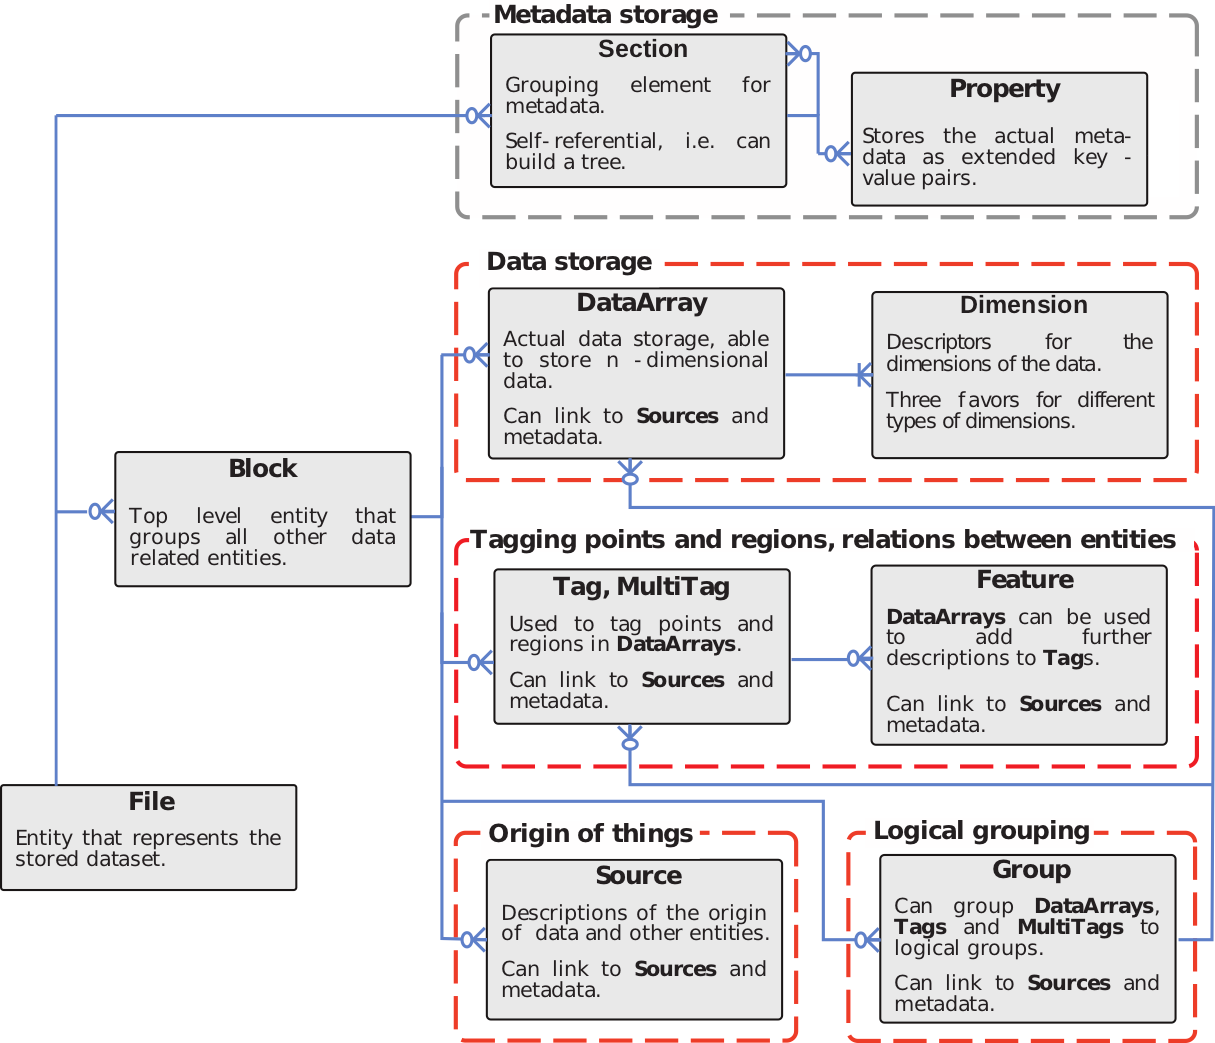
\includegraphics[width=0.9\textwidth]{./figures/introduction/data_model_brief_adapted}
 \caption[\software{Nix} model objects]{\software{Nix} model objects. The model consist of objects for storing data and metadata and relations between these. Metadata is captured in a \software{odML} based structure. Six objects are implemented to capture data and and relation between these. The main data object (\code{DataArray}) stores multidimensional data and captures the physical attributes of the data using \code{Dimension} objects. \code{Tag}s and \code{Multitag}s are used to label a subset of the data contained in an \code{DataArray} and can provide supplementary information using \code{Feature} objects. Furthermore, \code{Group} objects can be used to represent logical relations between objects and \code{Source} objects provide background information about the origin of the data. \code{Block}s and \code{File}s represent a complete dataset or file, respectively. Each of the data objects (except \code{Dimension}s) can link to a corresponding metadata \code{Section} providing additional metadata specific to that data object. Figure adapted from \software{Nix} documentation (\url{https://nixio.readthedocs.io/en/latest/data_model.html}).}
 \label{fig:intro_nix_model}
\end{figure}

\begin{figure}
 \centering
 \scalebox{0.45}{
 \includesvg[width=2\textwidth, pretex=\relscale{1}]{./figures/introduction/nix_example_merged_escus}}
 \caption[\software{Nix} model application examples]{\software{Nix} model application examples. The model can capture different varieties of data, e.g., electrophysiological recording traces (example 1) and imaging data (example 2). Both signals types can be mapped to the same types of objects of the \software{Nix} model. Figures from \software{Nix} the documentation (\url{https://github.com/G-Node/nix/wiki/The-Model}).}
 \label{fig:intro_nix_examples}
\end{figure}

The \software{Nix} repository is accompanied with an extensive wiki\footnote{\software{Nix} wiki, \url{https://github.com/G-Node/nix/wiki}} and documentation\footnote{\software{Nix} documentation, \url{https://nixio.readthedocs.io}} including tutorials and demos, providing detailed user-level documentation. Furthermore, the \software{Nix} model is natively integrated in the the electrophysiology recording system \software{RELACS}, the \software{EEGbase}\footnote{EEGbase, \url{http://eegdatabase.kiv.zcu.cz}, RRID:nif-0000-08190} a system for storage, management, sharing and retrieval of EEG data as well as \software{Neo}, a Python tool for standardized representation of electrophysiology data (\cref{sec:neo}).







\section{Thesis overview}
In \cref{sec:data} we describe two published datasets of a complex, electrophysiological experiment including an extensive metadata collection used in a collaborative setting. We describe the process of data and metadata preparation required for the data publication and discuss the pipeline used in this publication to identify strengths and shortcomings of the presented approach. In \cref{sec:metadata} we present odMLtables, a tool for facilitation of metadata collection compatible that emerged from the implementation of the previously presented pipeline. We demonstrate the embedding of odMLtables in a real-world metadata application and highlight the  features of the tool. \cref{sec:neo} complements the the previous section by introducing tools for standardized data representation and presents three example applications relevant in the context of data and metadata handling. \cref{sec:workflows} goes beyond the pipeline approach presented in \cref{sec:data} by introducing the concept of modern workflow management software for efficient organization and structuring of scientific projects. We demonstrate the integration of the previously presented tools in a systematic fashion using modern workflow management software to coordinate the application of data and metadata software in a neuroscientific project. Finally, in \cref{sec:discussion} we discuss the presented approaches and provide an outlook on future development of the tools and concepts.












































